\cotefile{156-8}
\scanpage{98}\mspage{89}
\uline{2 juillet}\qquad Déterminons maintenant les \uline{figures}. Tout drapeau $T$ \deleted{(\unsure{non} vide) de $L$} détermine une figure\deleted{\unsure{,|.}} $F_T$, savoir \deleted{\unsure{celle} \unsure{formée|que} \unsure{l'en}} 
\[
 F_T=\{X\in\unsure{M|\mathcal M}\mid X\ \text{\unsure{interstitiel|intersticiel} pour }T\},
\]
qu'on se représente graphiquement par
\figure{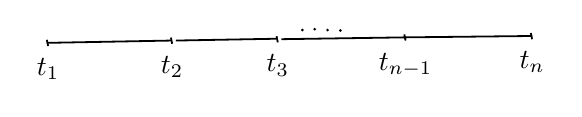
\begin{tikzpicture}[x=.78cm,y=.58cm,line width=.65pt]
\draw (0,0)--(2.0,.05) (2.08,.05)--(3.72,.09) (3.8,.08)--(5.82,.12)--(7.88,.15);
\foreach \x/\y/\lab in {0/0/{t_1},2.02/.05/{t_2},3.74/.08/{t_3},5.82/.12/{t_{n-1}},7.88/.15/{t_n}}{
 \draw (\x,\y-.07)--(\x-.02,\y+.065);
 \node[below=2pt] at (\x,\y) {$\lab$};}
\foreach \x/\y in {4.14/.28,4.34/.30,4.55/.28,4.76/.27}{\fill (\x,\y) circle (.53pt);}
\end{tikzpicture}}
(en ``oubliant'' les éléments de $L$ qui ne sont pas dans un des segments $[t_i,t_{i+1}]$, $1\leq i\leq n-1$. Les cas ``dégénérés'' sont \deleted{$T=\varnothing,\ F_{\varnothing}=\varnothing$}
% slanted
\margin{\uline{NB} $F_T$ détermine $T$ \unsure{par} $T=\delta F_T$}
\[
\begin{aligned}
 T=\varnothing &\Rightarrow F_T=\varnothing &&\text{graphisme :} && ?\\
 T=\{\deleted{\unsure{t}}\unsure{a|t}\} &\unsure{\Rightarrow|\mathrel{=}} F_T=\{P_{\deleted{\unsure{t}}\unsure{a|t}}\} &&\text{graphisme :} &&
 \vcenter{\hbox{\begin{minipage}{1.65cm}\figure{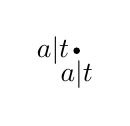
\begin{tikzpicture}[baseline]
 \node at (-.30,0) {$\deleted{\unsure{a|t}}$};
 \fill (0,0) circle (1.2pt) node[below] {$\unsure{a|t}$};
 \end{tikzpicture}}\end{minipage}}}\\
 T=\{\unsure{a|t},b\} &\Rightarrow F_T=\widetilde{S_{\unsure{a|t},\unsure{b|t_2}}} &&\text{graphisme} &&
 \vcenter{\hbox{\begin{minipage}{1.65cm}\figure{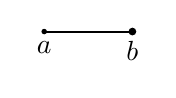
\begin{tikzpicture}
 \draw[line width=.7pt] (0,0) node[below] {$a$}--(1.12,0) node[below] {$b$};
 \fill (0,0) circle (1pt) (1.12,0) circle (1.4pt);
 \end{tikzpicture}}\end{minipage}}}
\end{aligned}
\]
après ça, on a
\figure{\begin{tikzpicture}[x=1cm,y=.65cm,line width=.65pt]
\draw[fill=white] (0,0) circle (1.3pt);
\draw (.075,0)--(1.55,.035) (1.64,.025)--(2.94,.035);
\draw[fill=white] (2.96,.035) circle (1.3pt);
\fill (1.54,.03) circle (1.2pt);
\node[below] at (0,0) {$a$};\node[below] at (1.55,0) {$b$};\node[below] at (3,0) {$c$};
\node at (7,.1) {etc.};
\end{tikzpicture}}

Sur l'ens des drapeaux \uline{non vides} $\mathrm{Drap}^{\unsure{*|\times}}(L)$ on met une relation d'ordre
\[
 T<T'\quad\text{\unsure{sss}}\quad \forall\,t\in T,t'\in T',\ \text{on a }t<t',
\]
% slanted
\margin{NB $T<T'$ (ou encore $T\parallel T'$ dans l'ens ordonné $\mathrm{Drap}^{*}(L)$) implique $T\cap T'=\deleted{\unsure{e}}\varnothing,\ T\cup T'\in\mathrm{Drap}^{*}(L)$}
qui nous permet de considérer des drapeaux de drapeaux.

\uline{Lemme} Soient $T,T'\in\mathrm{Drap}^{*}(L)$, pour que $F_T\parallel F_{T'}$ ($\Leftrightarrow F_T\mathrel{|\circ|}F_{T'}$) il \unsure{f. et s.} que $T\parallel T'$ \inserted{dans $\mathrm{Drap}^{*}(L)$} i.e. $\{T,T'\}\in\mathrm{Drap}^{*}(\mathrm{Drap}^{*}(L))$.
% archive sheet number: 98
\scanpage{99}\mspage{90}
\deleted{Si \unsure{donc} on}

\uline{Corollaire} Soit $\unsure{\mathscr{T}|\mathcal{T}}\unsure{\subset|\subseteq}\mathrm{Drap}^{\unsure{*|\times}}(L)$ un ens \unsure{de|des} drapeaux non vides. Pour que les figures $F_T$ ($T\in\mathscr{T}$) soient deux à deux disjointes, il f. et s. que $\mathscr{T}$ soit un drapeau de l'ens ordonné $\mathrm{Drap}^{*}(L)$.

Dans ce cas, on a donc une figure somme
\[
 F_{\mathscr{T}}\overset{\text{def}}{=}\bigcup_{T\in\mathscr{T}}F_T
\]
% slanted
\margin{Les $F_T$}
on retrouve $F_T$ comme cas particulier
\[
 F_T=F_{\{T\}}
\]

La figure vide correspond au cas $\mathscr{T}=\varnothing$.

\uline{Théorème} L'application
\[
\begin{aligned}
 &\mathscr{T}\longrightarrow F_{\mathscr{T}}\\
 &\mathrm{Drap}(\mathrm{Drap}^{*}(L))\longrightarrow
 \mathrm{Fig}\,\mathrm{fin}(\unsure{M|\mathcal M})=\unsure{\mathcal{F}|\mathscr{F}}
\end{aligned}
\]
est bijective.

Indication de la démonstration. Pour une figure donnée, on récupère les $F_T$ comme les ``composantes connexes'' (\deleted{\unsure{au|en}} \inserted{dans un} sens combinatoire \unsure{'}évident) de\deleted{\unsure{s}} $F$. Il \deleted{\unsure{f|y}} reste à voir que les composantes connexes d'une figure sont bien de la forme $\deleted{\unsure{E|F}}F_T$, puis utiliser le lemme précédent.
% archive sheet number: 99
\scanpage{100}\mspage{91}
\figure{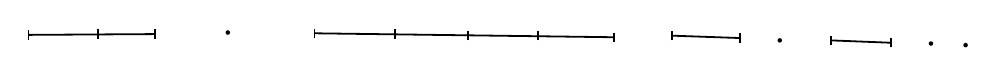
\begin{tikzpicture}[x=.1mm,y=.1mm,line width=.65pt]
\draw (0,1)--(161,2) (363,3)--(743,-2) (817,0)--(903,-3) (1019,-6)--(1095,-9);
\foreach \x/\y in {0/1,88/2,161/2,363/3,465/2,558/0,647/0,743/-2,817/0,903/-3,1019/-6,1095/-9}
 {\draw (\x,\y-6)--(\x,\y+6);}
\foreach \x/\y in {253/4,954/-6,1146/-10,1190/-12}{\fill (\x,\y) circle (2.9);}
\end{tikzpicture}}
exemple de figure -- les composantes connexes ``se suivent : la queue- leu- \unsure{leue|leu}''.
% margin note written sideways
\margin{\uline{Autre présentation} Se donner une figure \inserted{$F$} revient à se donner $\biggl\{$ a) un drapeau \deleted{$\unsure{D}$} \inserted{$F_0$} \deleted{\unsure{(}} (\deleted{$\unsure{=}$}$\delta F=\bigcup_{T\in\unsure{\mathscr T|\mathcal T}} T=F_0$)\unsure{,} b) une partie \deleted{$\unsure{P|F}$} $F_1$ de \deleted{\unsure{tout}} l'ens. $\mathrm{Int}_1(D)$ des segments interstitiels de $D$ (\unsure{ce sera} l'ensemble des segments de $F$ (ou au choix, son complémentaire -- les segments interstitiels \uline{de la figure}}

Il faudrait déterminer le\deleted{\unsure{s}} \deleted{\unsure{comp}} \deleted{\unsure{santes}} support d'une figure. Pour y arriver, on aura à utiliser

\uline{Hypothèse} H) \deleted{Pour tout élément $a$ de $L$, si \unsure{$a$ n'est pas un plus} \unsure{grand}} \inserted{a) Tout élément minimal de $L$ est un plus petit élément} \deleted{\unsure{ce}} ou \unsure{encore|aussi} : si $L$ n'a pas de plus petit élément, alors pour tout $a\in L$, existe $x\in L$ tel que $x<a$.

b) hypothèse duale.
% margin note written sideways
\margin{\uline{NB} Donc pour $D$ donné avec $\mathrm{card}\,D=n$, il y aura $2^{n-1}$ figures qui lui correspondent.}
% margin note written sideways
\margin{\unsure{ens} des sommets \uline{de $F$}}

On aura besoin de cette hypothèse dès \inserted{le lemme 1}

\deleted{\uline{Lemme 1} Soient $X,Y\in\unsure{M|\mathcal M}$ tels que $X\parallel Y$, et soit $\Phi\unsure{\subset|\in}\mathrm{Omb}\,X$, $\Psi\subset\mathrm{Omb}\,Y$. Alors}
\[
 \deleted{\mathrm{Supp}^{\circ}(\Phi\cup\Psi)=\mathrm{Supp}^{\circ}(\Phi)}
\]

\uline{Lemme 1} Soit $X\in M$. Alors
\[
\begin{aligned}
 \mathrm{supp}(X)\bigl(\overset{\text{def}}{=}\mathrm{supp}^{\circ}(\widetilde X)\bigr)
 &=\mathrm{Omb}(X)=\{ \deleted{\unsure{Y}}Z\in M\mid\\
 &\hspace{22mm}|\deleted{\unsure{Y}}Z|\subset |X|\}
\end{aligned}\tag*{(1)}
\]
% slanted
\margin{On peut y mettre aussi \unsure{(NB)|(1)|Obs} $\mathrm{supp}^{\circ}(X)=\mathrm{Omb}^{\circ}(X)$ $\deleted{\unsure{=}}\overset{\text{def}}{=}\{Y\in M\mid Y\deleted{\unsure{L}}\unsure{\overset{\circ}{\ll}_{1}|\ll_{1}}X\}$}
L'inclusion $\mathrm{Omb}(X)\subset\mathrm{supp}(X)$ est triviale, c'est l'autre inclusion qui l'est un peu moins.
% archive sheet number: 100
\scanpage{101}\mspage{92}
\margin{$\mathrm{Supp}$}
\uuline{Cor 1}
\[
 \mathrm{Supp}(\{P_a\})\inserted{=\mathrm{Supp}^{\unsure{\bullet|\circ}}(\{P_a\})}=\{P_a\}
\]

\uline{Cor. 2}
\[
 \mathrm{Supp}(\{S_{a,b}\})=
 \left\{\deleted{\unsure{X|P}}Z\ \middle|\
 \begin{aligned}&Z=P_x\ \text{avec }a\leq x\leq b\\
 &\text{ou }Z=S_{x,y}\ \text{avec }a\leq x<y\leq b\end{aligned}
 \right\}
\]

\uline{Cor. 3}
\[
\begin{aligned}
 \mathrm{Supp}^{\circ}\{S_{ab}\}
 &=\deleted{\unsure{\{}}\inserted{\mathrm{Omb}^{\circ}(S_{ab})=}
 \mathrm{Supp}(\{S_{ab}\})\setminus\underset{\inserted{\{P_a,P_b\}}}{\underline{\unsure{\partial|\delta}S_{ab}}}\\
 &=\left\{Z\ \middle|\
 \begin{aligned}&Z=P_x\ \text{avec }a<x<b\\
 &\overset{\text{ou}}{Z}=S_{x,y}\ \text{avec }a\leq x<y\leq b\end{aligned}\right\}
 \deleted{=\mathrm{Omb}^{\circ}(S_{ab})}
\end{aligned}
\]

On trouve de \={m}

\uline{Cor. 4}
\[
\begin{aligned}
 \mathrm{Supp}^{\circ}(\{S_{a,b},P_a\})&=\deleted{\unsure{S}}\mathrm{Omb}^{\circ}(S_{ab})\cup\{P_a\}\\
 \mathrm{Supp}^{\circ}(\{S_{ab},P_b\})&=\mathrm{Omb}^{\circ}(S_{ab})\cup\{P_b\}
\end{aligned}
\]

\uline{Démonstration des} \uline{Cor 1 et 2}. (\unsure{équivalents|équivalente|équivalent} au lemme 1).

\deleted{On a, par définition}
\[
\begin{aligned}
 &\deleted{\mathrm{Cosupp}^{\circ}(P_a)=L_{<a}\cup L_{>a}=\{x\in L\mid x<a\text{ ou }x>a\}}\\
 &\deleted{\mathrm{Supp}^{\circ}(P_a)=\mathrm{supp}(P_a)=\mathrm{cosupp}^{\circ}(\mathrm{cosupp}^{\circ}(P_a))}
\end{aligned}
\]
\deleted{Soit $X\in\mathrm{supp}^{\circ}(P_a)$. On a donc}
\[
 \deleted{X\mathrel{\unsure{\vert\cdot\vert|\vert\circ\vert}}x\qquad\forall\,x\in\mathrm{cosupp}^{\circ}(P_a)}
\]
\deleted{Si $a$ n'est pas plus grand \unsure{él|1}}

\uline{Cor. 1} Soit $X\in\mathrm{supp}^{\circ}(P_a)$ ($=\mathrm{supp}(P_a)$), i.e. $X\mathrel{|\circ|}Y$, $\forall\,Y\in\mathrm{cosupp}^{\circ}(P_a)$.

Si $a$ est un plus petit ou plus grand \unsure{élt} alors $\mathrm{cosupp}^{\circ}(P_a)=\unsure{M|\mathcal M}-\{P_a\}$ ( tout $\unsure{Y|X}\in\unsure{\acute M|M}$
% archive sheet number: 101
\scanpage{102}\mspage{93}
distinct de $P_a$ est $\mathrel{|\circ|}$ \unsure{à|:} $P_a$), d'où résulte aussitôt (à cause de l'antiréflexivité de $\mathrel{|\circ|}$) que $\mathrm{supp}^{\circ}(P_a)=\{P_a\}$. Si $a$ n'est \deleted{\unsure{p}}\unsure{ni|pas} plus petit ni plus grand élément, soient
\[
 \deleted{\unsure{x<a}}\qquad x<a<y\qquad .
\]
Alors $\deleted{\unsure{\exists|Z}}S_{x,a}\in\mathrm{cosupp}^{\circ}(P_a)$, donc $X\mathrel{|\circ|}S_{x,a}$, \deleted{donc} $\delta X\geq a$ ou $\delta X\leq x$. Mais on ne peut avoir $\delta X\leq x$, car on aurait $X\mathrel{|\circ|}a$ i.e. $X\in\mathrm{cosupp}^{\circ}(P_a)$, ce qui contredit $X\in\mathrm{supp}^{\circ}(P_a)$ (vu l'\unsure{antiréflexivité|antiréflexité}) :
\[
 \mathrm{cosupp}^{\circ}(\Phi)\cap\mathrm{supp}^{\circ}(\deleted{\unsure{\Psi}}\Phi)=\varnothing,\quad\text{pour tte partie}
\]
$\Phi$ de $\unsure{M|\mathcal M}$). Donc $\delta X\geq a$. L'\deleted{\unsure{m\={m}|=}}argument symétrique, utilisant $S_{a,y}$ \unsure{ald|.ld} $S_{xa}$, donnera $\delta X\leq a$, d'où la conclusion.

\uline{Cor. 2} Raisonnement analogue ; \deleted{\unsure{on}} \inserted{On} \deleted{Si $a$ est un \unsure{p}} prouve successivement
\[
 \delta X\geq a,\quad\text{puis }\delta X\leq b
\]
en distinguant, pour la première, le cas où $a$ est un plus petit élément (\unsure{trivial}) et le cas où il ne l'est pas, donc $\exists\,x$
\[
 x<a<b
\]
et on aura $S_{x,a}\in\mathrm{cosupp}^{\circ}(S_{ab})$ donc $X\mathrel{|\circ|}S_{x,a}$ donc $\delta X\leq x$ ou $\delta X\geq a$, et le premier cas est exclu comme devant \unsure{entrainer|entraîner} $X\mathrel{|\circ|}\unsure{\widetilde S_{ab}|S_{ab}}$, \unsure{exclu,|exclu.}
% archive sheet number: 102
\scanpage{103}\deleted{\unsure{93|95}}\mspage{94.}
Cas où on ne fait pas l'hyp. par exemple
% slanted
\margin{\uline{\unsure{Cancelé|Cancellé|Calculé}}}
\diagram{\begin{tikzcd}[ampersand replacement=\&,row sep=small,column sep=small]
 \& b \&\\
 a\arrow[ur,line width=.95pt] \& \& \unsure{c|e}\arrow[ul]
\end{tikzcd}}
\[
\begin{aligned}
 \mathrm{cosupp}^{\circ}(\{P_a\})&=\{P_b\unsure{\}}\unsure{,|;}\\
 \mathrm{supp}^{\circ}(\{P_a\})&=\{P_a,P_{\unsure{c|b}},\inserted{\deleted{\unsure{P}}\unsure{S|P}_{ab},S_{c,b}}\}\ne\{P_a\}
\end{aligned}
\]
\[
 \unsure{\downarrow|J}=\mathrm{cosupp}^{\circ}(P_b)=\unsure{M|\mathcal M}\setminus\{P_b\}
\]
\[
\begin{aligned}
 \mathrm{cosupp}^{\circ}(\deleted{\unsure{\{P_a\}}}\widetilde{S_{ab}})&=\varnothing\\
 \mathrm{supp}^{\circ}(\widetilde{S_{ab}})&=M\ne\mathrm{Omb}(S_{ab})
\end{aligned}
\]
(NB $M=\mathrm{Omb}(S_{ab})\amalg\{S_{c,b},P_c\}$

ici $\mathrm{card}\,M=5$

Par contre, pas de Pb avec
\diagram{\begin{tikzcd}[ampersand replacement=\&,row sep=small,column sep=small]
 \& b \&\\
 a\arrow[ur] \& \& d\arrow[ul]\\
 \& c\arrow[ul]\arrow[ur] \&
\end{tikzcd}}
p. ex.

\[
\begin{aligned}
 &\deleted{\mathrm{cosupp}^{\circ}P_a=\{P_b,P_c\},S_{ab},S_{ca}\}}\\
 &\deleted{\mathrm{supp}^{\circ}P_a=}
\end{aligned}
\]
\deleted{\uline{Lemme 2} Soient} $\deleted{\Phi\subset M,\ \Psi\subset M\ \unsure{t}}$ \deleted{$X,Y\in M$ avec $X\parallel Y$, et soit $\Phi\subset\mathrm{Omb}(X)$,} $\deleted{\unsure{\Psi}}$ \deleted{($=\mathrm{supp}\,\widetilde X$ par lemme 1), $\Psi\subset\mathrm{Omb}(Y)$ ($=\mathrm{supp}\,\widetilde Y$). Alors}
\[
 \deleted{\mathrm{supp}^{\circ}(\Phi\cup\Psi)=\mathrm{supp}^{\circ}\Phi\cup\mathrm{supp}^{\circ}\Psi.}
\]

% slanted
\margin{4 \uline{juillet}}
Détermination des \unsure{préfigures|profigures}, ou ensembles constructibles \unsure{dans|de ce|de} $M$.

\deleted{Les} Pour la relation d'ordre induite, une préfigure se décompose en composantes connexes. Les composantes connexes \inserted{(ou préfigures connexes)} sont des types \unsure{suivant|suivants} 

\deleted{a) Dim 0}
\figure{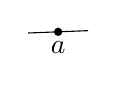
\begin{tikzpicture}[baseline]\fill (0,0) circle (1.5pt) node[below] {$\deleted{a}$};
\draw (-.38,-.015)--(.38,.015);\end{tikzpicture}}
\deleted{$\Phi=\{P_a\}$ c'est une figure \unsure{fermée|ferm}}

\deleted{b) Dim 1\qquad b) Figure}
\figure{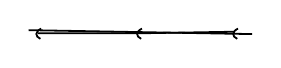
\begin{tikzpicture}[line width=.65pt]\draw (0,0)--(1.28,0)--(2.5,.02);
\foreach \x in {0,1.28,2.5}{\draw (\x+.04,.06) .. controls (\x-.04,.02) and (\x-.04,-.04) .. (\x+.03,-.07);}
\draw (-.12,.04)--(2.72,-.01);\end{tikzpicture}}
% archive sheet number: 103
\scanpage{104}\mspage{95}
% archive sheet number: 104
a) \unsure{préfigures|Préfigures} \uline{\unsure{fermées|fermée}} $0$-connexes \inserted{$=$ figures $0$-connexes} -- déterminées par les éléments de $\mathrm{Drap}^{\unsure{*|\times}}(\unsure{L|\mathcal L})$, cf plus haut

b) Figures \deleted{\unsure{f}} ouvertes $0$-connexes : \deleted{\unsure{cas de}} elles sont données par $\deleted{\unsure{D}}T\in\mathrm{Drap}^{*}(L)$ \uline{$\mathrm{card}\,\deleted{\unsure{D}}T\geq 2$}, et une partie de
\[
\begin{aligned}
 \partial F_T\overset{\text{def}}{=}\unsure{\partial|\delta}T
 &=\{\text{ensemble formé du plus}\\
 &\qquad\text{petit et du plus grand}\\
 &\qquad\text{élément de }T=F_0\}
\end{aligned}
\]
\[
 \Phi=F\setminus\partial\unsure{F|T}
\]
\margin{\uline{NB} On a finalement identifié les $P_a$ aux $a$, i.e. $\unsure{M|\mathcal M}_0$ à $L$ \ldots}

c) Cas général : on se donne une partie $\deleted{\unsure{\beta}}\alpha$ de $\partial F$, et on prend
\[
 \Phi=F\setminus\alpha
\]

\uline{Ex} Segments fermé, semi-ouvert, ouvert (\deleted{\unsure{cas}} $\mathrm{card}\,T=2$)

\deleted{\unsure{B|D}}Soit $\text{PréFig conn}(M)$ l'ensemble des préfigures connexes, qu'on vient d'expliciter, identifié aux couples $(T,\alpha)$, $T\in\mathrm{Drap}^{*}(L)$, $\alpha\in\partial T$ (\deleted{frontière}''bord de la figure \inserted{connexe} $F_T$ ; \uline{NB} si $F_T=\{P_x\}$, on \deleted{\unsure{aura}} \inserted{prendra} $\partial F_T=\varnothing$).
% slanted
\margin{On pose $F=\overline{\Phi}$ (plus petite figure \deleted{fermée} \unsure{contenant} la préfigure), $\partial F=\partial\Phi$}

\deleted{On va définir \unsure{sur|dans}}
\[
 \deleted{\text{Préfigconn}(M)}
\]
\deleted{une relation d'ordre} $\deleted{\inserted{<}}$, \deleted{en écrivant}
\[
 \deleted{\Phi<\Phi'\Longleftrightarrow}
 \left\{\begin{aligned}
 &\deleted{\text{a) pour tout }X\in\Phi,X'\in\Phi',\ \text{on a}}\\
 &\deleted{X\underset{\mathrm{pos}}{<}X'\ \text{\unsure{au sens}}}\quad\deleted{\text{cf plus bas}}\\
 &\deleted{\text{\unsure{b)}}}\quad\deleted{-\ \text{\unsure{cel|cela|ceci} implique }\mathrm{card}\,\partial\Phi\cap\partial\Phi'\leq1}\\
 &\deleted{\text{b) Si }x\in\partial\Phi\cap\partial\Phi',\ \text{on a }x\notin\Phi,x\notin\Phi'}
 \end{aligned}\right.
\]
\margin{\uline{NB} b) \unsure{indique|implique} que si $\Phi$ de dim $0$ i.e $\Phi=\{P_a\}$ \inserted{alors $\unsure{\partial|\delta}$}}
\scanpage{105}
\mspage{96}

Soit $\Phi$ une préfigure, $F$ la figure engendrée (on posera $F=\overline{\Phi}$, c'est bien l'adhérence de $\Phi$ pour $\leq$ sur $\unsure{M|\mathcal M}$), on pose
\[
\begin{aligned}
\delta\Phi\overset{\mathrm{def}}{=}\delta F=F\cap M_0
  =\bigl\{a\in L\mid{}& P_a\in F,\ \text{i.e.}\\[-2pt]
  &\exists X\in\Phi,\ P_a\leq X\bigr\}
\end{aligned}
\]
\[
\begin{aligned}
\deleted{\partial\Phi\overset{\mathrm{def}}{=}\partial F=}
&\ \deleted{\biggl\{\varnothing\ \text{si }\mathrm{card}\,\delta F\leq1}\\
&\ \deleted{\text{\unsure{``bord''|bord''}}}\\
&\ \deleted{\text{ens. formé des }\unsure{\text{plus petit}|\text{plus petits}}\text{ et }\inserted{\text{``extrémités''}}\text{ de }\delta F}\\
&\quad\deleted{\text{\unsure{du plus|des plus}}}
\end{aligned}
\]

\uline{NB} $\delta\Phi=\delta F\in\mathrm{Drap}^{\unsure{*|\times}}(L)$, ens. des \deleted{\unsure{points|points pr.}} \deleted{\unsure{principaux}} \uline{sommets} \deleted{pour $\Phi$, \unsure{et} pour $F$} \uline{de la préfigure $\Phi$}. Il est $\varnothing\deleted{\unsure{=|\ne}}$ \unsure{sss|ss} $\Phi=\varnothing$, \deleted{vide} de card 1 sss. $\Phi=\deleted{\unsure{\varnothing|P_a}}\{P_a\}$, auquel cas $\Phi=F$.

% slanted
\margin{Attention, si $a$ est un sommet de $\Phi$, on n'a pas nécessairement $P_a\in\Phi$, ex : $\Phi=\{S_{ab}\}$}

\uline{Cas $\Phi$ connexe}
\margin{\uline{bord de $\Phi$}\\ $\partial\Phi=\partial F$}
\[
\partial\Phi\overset{\mathrm{def}}{=}
\left\{\begin{aligned}
&\text{a) }\varnothing\ \text{si }\deleted{\unsure{\delta\Phi=\varnothing|\Phi=\varnothing}}\mathrm{card}\,\delta\Phi\leq1,\quad\text{i.e. }\Phi=\varnothing\ \text{ou }\{P_a\}\\
&\text{b) ``bord de }\delta\Phi\text{'' }\deleted{\text{\unsure{si|déf.}}}\mathrm{card}\,\delta\Phi\geq2,\quad\text{i.e.}\\
&\qquad\text{ens. formé des extrémités du}\\
&\qquad\text{drapeau }\deleted{\Phi}\delta\Phi\quad\text{(plus petit et}\\
&\qquad\text{plus grand élément)}
\end{aligned}\right.
\]
ainsi, $\partial\Phi=\varnothing$ ou $\in\mathrm{Drap}_2(L)$.

\[
\left[\ \text{\uline{Cas $\Phi$ connexe}}\quad
\Phi^{\unsure{\bullet|'}}=
\left\{\begin{aligned}
&\partial\Phi\ \text{ si }\mathrm{card}\,\delta\Phi\geq 2\\
&\{a\}\ \text{ si }\Phi=\{P_a\}\quad\text{i.e. }\mathrm{card}\,\delta\Phi=1\\
&\varnothing\ \text{ si }\Phi=\varnothing\quad\text{i.e. }\mathrm{card}\,\delta\Phi=0
\end{aligned}\right.\ \right]
\]
% slanted
\margin{\uline{définition} \uline{correcte}, à cause des plus petits ou plus \unsure{gds|grds} él. de $L$, mais on \unsure{ne va pas|va pas} l'utiliser}

% slanted
\margin{$\partial\Phi=\{a\in L\mid\deleted{\unsure{a\notin\Phi|a\in\Phi}},\ \mathrm{ordre}_{a}\deleted{\unsure{\text{ de }\Phi\,a|\text{ de }\Phi}}\,\unsure{(\text{pour}|(\text{disons}}\ \deleted{\text{\unsure{de}}}\overline{\Phi})=1\}$\\
On pose $\Psi\inserted{\text{préfigure}}\in M$, \uline{$a\in L$, on pose}\\
$\mathrm{ordre}(a,\Psi)=\mathrm{card}(\{X\in M_1\cap\Psi\mid a\unsure{\in|\triangleleft}\partial X\}$\\
(cet ordre est $0,1$ ou $2$)\\
$0$ point extérieur (si $a\in\Psi$) ou isolé (si $a\notin\Psi$)\\
$1$ point bord\\
$2$ point frontière \unsure{interne|intérieur} (si $a\notin\Psi$) ou point \deleted{\illegible{1}} \inserted{de} \unsure{rédondance|redondance|de charnière} (ou de morcellement) si $a\in\Psi$}

On pose, pour $\Phi$ pas néc. connexe
\[
\begin{aligned}
\partial\Phi&=\bigcup\partial\Phi_i & &\text{où les }\Phi_i\text{ sont les}\\
\Phi^{\bullet}&=\bigcup\Phi_i^{\bullet} & &\text{comp. connexes.}
\end{aligned}
\]

\uline{Ex} $\Phi=\{S_{ab},S_{bc},\deleted{\}}P_d\}$ \inserted{où $a<b<c<d$.} comp. connexes $S_{ab},S_{bc},\inserted{P_d}$
\[
\begin{aligned}
\delta\Phi&=\{a,b,c,d\}\\
\partial\Phi&=\{a,b,c\}\\
\Phi'&=\{a,b,c,d\}
\end{aligned}
\]
% archive sheet number: 105
